\documentclass[10pt,twocolumn,letterpaper]{article}

% ---------------------------------------------------------------
% Include basic CVPR package in rebuttal mode

\usepackage[rebuttal]{cvpr}

% ---------------------------------------------------------------
% Other packages

\usepackage{titlesec}

\titlespacing*{\paragraph}{1pc}{2pt}{0.6em}

% Commonly used abbreviations (\eg, \ie, \etc, \cf, \etal, etc.)
\usepackage{eccvabbrv}

% Include other packages here, before hyperref.
\usepackage{graphicx}
\usepackage{booktabs}
\usepackage{multirow}

\usepackage[T1]{fontenc}
\usepackage{tikzsymbols}

% The "axessiblity" package can be found at: https://ctan.org/pkg/axessibility?lang=en
\usepackage[accsupp]{axessibility}  % Improves PDF readability for those with disabilities.

\usepackage[table]{xcolor}


% Reviewer colors
\definecolor{revone}{HTML}{FF7F00}    % orange
\definecolor{revtwo}{HTML}{0000CC}    % blue
\definecolor{revthree}{HTML}{008C8C}  % teal
\definecolor{revfour}{HTML}{7A3DB8}   % purple

\usepackage{array}
\definecolor{clsbg}{RGB}{232,242,255}
\definecolor{segbg}{RGB}{232,248,238}
\definecolor{actbg}{RGB}{255,241,224}

\definecolor{clstext}{RGB}{30,90,170}
\definecolor{segtext}{RGB}{30,130,70}
\definecolor{acttext}{RGB}{190,105,20}

\definecolor{trainbg}{RGB}{232,242,255}
\definecolor{inferbg}{RGB}{255,241,224}

\definecolor{traintext}{RGB}{30,90,170}
\definecolor{infertext}{RGB}{190,105,20}

\usepackage{caption}
\captionsetup{font=footnotesize}

\newcommand{\methodcolor}[0]{green!20}

% Helper
\newcommand{\reviewertag}[2]{%
  \textcolor{#1}{\textbf{#2}}%
}

% Usage: \R1, \R2, \R3, \R4
\DeclareRobustCommand{\R}[1]{%
  \ifcase#1\relax
    \PackageError{reviewers}{Reviewer number must be 1--4}{}%
  \or
    \reviewertag{revone}{QH3c}%
  \or
    \reviewertag{revtwo}{yCUw}%
  \or
    \reviewertag{revthree}{LjJR}%
  \or
    \reviewertag{revfour}{SXMH}%
  \else
    \PackageError{reviewers}{Reviewer number must be 1--4}{}%
  \fi
}

\usepackage{pifont} % if you use \cmark \xmark
\newcommand{\cmark}{\ding{51}}
\newcommand{\xmark}{\ding{55}}


\setlength{\textfloatsep}{6pt plus 1pt minus 2pt} % space between top/bottom floats and text
\setlength{\floatsep}{6pt plus 1pt minus 2pt}     % space between two floats
\setlength{\intextsep}{6pt plus 1pt minus 2pt}    % space around [h] in-text floats

% Caption spacing
\setlength{\abovecaptionskip}{2pt}  % space above caption
\setlength{\belowcaptionskip}{2pt}  % space below caption, important for tables with caption above

% ---------------------------------------------------------------
% Hyperref package
% If you comment hyperref and then uncomment it, you should delete
% egpaper.aux before re-running latex.  (Or just hit 'q' on the first latex
% run, let it finish, and you should be clear).

\definecolor{eccvblue}{rgb}{0.12,0.49,0.85}
\usepackage[pagebackref,breaklinks,colorlinks,citecolor=eccvblue]{hyperref}


% ---------------------------------------------------------------
% If you wish to avoid re-using figure, table, and equation numbers from
% the main paper, please uncomment the following and change the numbers
% appropriately.
%\setcounter{figure}{2}
%\setcounter{table}{1}
%\setcounter{equation}{2}

% If you wish to avoid re-using reference numbers from the main paper,
% please uncomment the following and change the counter for `enumiv' to
% the number of references you have in the main paper (here, 6).
%\let\oldthebibliography=\thebibliography
%\let\oldendthebibliography=\endthebibliography
%\renewenvironment{thebibliography}[1]{%
%     \oldthebibliography{#1}%
%     \setcounter{enumiv}{6}%
%}{\oldendthebibliography}


% ---------------------------------------------------------------
% TODO REBUTTAL: Please enter paper ID
\def\paperID{14503} % *** Enter the paper ID here
\def\confName{ECCV}
\def\confYear{2026}

\begin{document}

% ---------------------------------------------------------------
% TODO REBUTTAL: Paper title is not required
% \title{\LaTeX\ Guidelines for Author Response}  % **** Enter the paper title here

%\maketitle
\thispagestyle{empty}
\appendix


We thank the reviewers for their thoughtful feedback and for recognizing the importance of the problem (\R1, \R3, \R4), the elegance and practicality of the method (\R1, \R2, \R4), and the breadth of the evaluation (\R1, \R2, \R3).
The main concerns are the precision of claims (\R1, \R4), the role of the training objective and architecture (\R1, \R3, \R4), and confusion about SteerViT variants (\R2), which we address below.

\paragraph{Preservation of Feature Quality.} \R4 notes that claims about preserving representation quality are overstated given the reported degradation. Post deadline, we identified an issue causing the CLS token and normalization layers to be optimized. Freezing both brings SteerViT much closer to its vanilla backbone without affecting steerability. 
As requested by \R2, we consider additional downstream tasks in Tab.~\ref{tab:feature_preservation}. Here, SteerViT closely tails DINOv2 (87.0 vs. 88.1), confirming that no significant decline of transfer ability occurs. 
We will update the numbers in the paper. 



\begin{table}[b]
\centering
\footnotesize
\setlength{\tabcolsep}{3.5pt}
\renewcommand{\arraystretch}{0.92}

\caption{
SteerViT maintains 98.8\% of DINOv2's avg. performance across
\textcolor{clstext}{classification},
\textcolor{segtext}{segmentation}, and
\textcolor{acttext}{action recognition} downstream tasks.
% With $\omega{=}0.0$, SteerViT is identical to DINOv2.
Setting $\omega{=}0.0$ (post-hoc gate steering) recovers DINOv2 performance. 
}
\label{tab:feature_preservation}
\resizebox{\linewidth}{!}{
\begin{tabular}{@{}l
>{\columncolor{clsbg}}c
>{\columncolor{clsbg}}c
>{\columncolor{clsbg}}c
>{\columncolor{segbg}}c
>{\columncolor{segbg}}c
>{\columncolor{actbg}}c
>{\columncolor{actbg}}c c@{}}
\toprule
\textbf{Model}
& \textcolor{clstext}{Birds}
& \textcolor{clstext}{Cars}
& \textcolor{clstext}{Dogs}
& \textcolor{segtext}{ADE20k}
& \textcolor{segtext}{City.}
& \textcolor{acttext}{UCF101}
& \textcolor{acttext}{HMDB51} & Avg. \\
\midrule
DINOv2                  & \textbf{94.7} & \textbf{83.8} & 89.1 & 53.7 & 52.8 & \textbf{92.3} & \textbf{62.3}  & \textbf{88.1}\\
% SteerViT $\alpha_\ell^{0.0}$ & \textbf{94.7} & \textbf{83.8} & 89.1 & 53.7 & 52.8 & \textbf{92.3} & \textbf{62.3}  & \textbf{88.1}\\
SteerViT & 91.2 & 77.7 & \textbf{94.3} & \textbf{55.4} & \textbf{53.8} & 89.4 & 60.0  & 87.0 \\
\bottomrule
\end{tabular}}
\end{table}

\paragraph{Generalization Claims.}
We agree with \R1 and \R4 that some claims were too broad. 
``Zero-shot generalization'' was used to highlight the ability of SteerViT representations to transfer to tasks different from the referential segmentation training objective. 
For PODS, we will follow \R1's suggestion and describe the result as an application of frozen SteerViT features.
For anomaly segmentation, ``zero-shot'' follows the AS literature since no target-dataset tuning is used. However, we will revise ``matches or outperforms dedicated approaches'' to more precisely state that SteerViT is competitive, outperforming dedicated AS methods in 10/18 settings (Tab.~7), but not dominating all baselines.

\paragraph{Late vs. Early Fusion.}
We agree with \R1 that early fusion should not be framed as a strict desideratum. As noted by \R3, our late-fusion ablation is a strong baseline, achieving similar steerability on CORE for DINOv2. However, Tab.~3 also shows that early fusion becomes more important when steering requires fine-grained language-vision grounding (e.g. 53.4 vs 45.3 on PODS). Moreover, SigLIP and MAE benefit more strongly from early fusion, as shown in Tab.~4. 
We will therefore revise the introduction not to claim that late fusion cannot steer features, but that early fusion provides a more robust mechanism across tasks and backbones.
% We will therefore revise the introduction to express that early fusion provides a more robust mechanism across tasks and backbones.
% We will revise the introduction accordingly.


\paragraph{Design Choices.}
Addressing \R1 and \R4, we ablate data scale under a fixed 200k-iteration budget (Tab.~\ref{tab:data_arch_ablation}). Even 25\% data reaches 95.3 CORE and 55.6 PODS, close to the full-data model, suggesting that gains are not simply due to the scale of grounding data. To address \R1’s architectural concern, ungated and sigmoid-gated variants remain competitive, but tanh gating gives the best balance. Adding an FFN does not help, supporting our lightweight default design.

% \section{Efficiency and Resource Requirements}

\paragraph{Efficiency and Resource Requirements.} Based on feedback from reviewers \R1 and \R4, we measure and report efficiency of SteerViT and baselines in Tab.~\ref{tab:efficiency}. 
SteerViT optimizes 21.2M parameters for ${\sim}$84 H100 hours.

% \section{Individual Responses}
\paragraph{MLLM-based Embedding Models.}
Following \R3, we evaluated Qwen3-VL-Embedding-2B and found improvements over the non-embedding variant in global representation quality ($+2.2$) and CORE steerability ($+12.1$).
% FG-CLS    CORE    ADE20k
% 91.182	64.918	37.369 (Qwen3-VL-2B)
% 93.408	77.038	37.072 (Qwen3-VL-Embedd-2B)


\begin{table}[t]
\centering
\footnotesize
\setlength{\tabcolsep}{3pt}

\caption{
Compute and data efficiency during \textcolor{traintext}{MM training} and
\textcolor{infertext}{inference}.
Averaged over 256 images (336x336) encoded in batches of 16 on a single A100 GPU with prompts of 20 words. % (avg. of PODS descriptions). 
``Tuned'' denotes trainable modules.
}
\label{tab:efficiency}

\resizebox{\linewidth}{!}{%
\begin{tabular}{@{}l c
>{\columncolor{trainbg}}c
>{\columncolor{trainbg}}c
>{\columncolor{inferbg}}r
>{\columncolor{inferbg}}r
>{\columncolor{inferbg}}r@{}}
\toprule
Name & Params
& \textcolor{traintext}{Tuned}
& \textcolor{traintext}{Samples}
& \shortstack[c]{\textcolor{infertext}{Compute}\\[-1pt]{\scriptsize GFLOPS/img}}
& \shortstack[c]{\textcolor{infertext}{Latency}\\[-1pt]{\scriptsize ms/img}}
& \shortstack[c]{\textcolor{infertext}{Memory}\\[-1pt]{\scriptsize peak GiB}} \\
\midrule
% CLIP          & 150M & all & 400M  & 81.4   & 5.5  & 1.1  \\
DINOv2        & 86M  & n/a & n/a   & 98.6   & 6.6  & 1.0  \\
\rowcolor{\methodcolor}
SteerViT      & 465M & GCA & 2.28M & 133.8  & 9.5  & 3.0  \\
% GroundDINO    & 172M & all & 5.4M  & 515.0  & 59.7 & 16.3 \\
SAM3          & 840M & all & 146M  & 556.0  & 35.1 & 5.3  \\
InternVL3-1B  & 938M & all & n/r   & 931.8  & 8.3  & 3.9  \\
InternVL3-2B  & 2.1B & all & n/r   & 1591.0 & 12.2 & 6.3  \\
\bottomrule
\end{tabular}%
}
\end{table}




% #############

% Optional color definitions, if not already defined elsewhere.
% Adjust to match your existing palette.
\definecolor{databg}{HTML}{EAF3FF}
\definecolor{datatext}{HTML}{1F5FA8}
\definecolor{archbg}{HTML}{FFF2E6}
\definecolor{archtext}{HTML}{B45F06}

\begin{table}[t]
\centering
\footnotesize
\setlength{\tabcolsep}{3pt}
\renewcommand{\arraystretch}{0.92}

\caption{
Ablating \textcolor{datatext}{dataset size} and \textcolor{archtext}{design choices}.
The default uses early fusion, tanh gating, and no FFN with 100\% data trained for 200k iterations.
}
\label{tab:data_arch_ablation}

\resizebox{\linewidth}{!}{%
\begin{tabular}{@{}l c c
                c c c c c@{}}
\toprule
\textbf{Setting}
& \shortstack[c]{Gate}
& \shortstack[c]{FFN}
& FG-CLS
& ADE20k
& CORE
& PODS
& MVTec \\
\midrule
\rowcolor{databg}
Data 25\%        & tanh    & \xmark & 88.4 & 53.2 & 95.3 & 55.6 & 77.4 \\
\rowcolor{databg}
Data 50\%        & tanh    & \xmark & 88.0 & 54.0 & 95.2 & 52.8 & 82.6 \\
\rowcolor{\methodcolor}
Default          & tanh    & \xmark & \textbf{89.5} & \textbf{55.3} & \textbf{95.5} & 55.4 & 77.9 \\
\addlinespace[1pt]
\rowcolor{archbg}
No gating        & none    & \xmark & 88.2 & 54.7 & 95.0 & 56.0 & \textbf{82.9} \\
\rowcolor{archbg}
Sigmoid gate     & sigmoid & \xmark & 88.1 & 55.2 & 95.3 & \textbf{58.9} & 82.3 \\
\rowcolor{archbg}
With FFN         & tanh    & \cmark & 87.6 & 55.0 & 95.1 & 53.7 & 82.4 \\
\bottomrule
\end{tabular}%
}
\end{table}

% #############




\paragraph{Prompt Complexity.}
Reviewer \R4 suggests more analysis on prompt complexity.
To test generalization beyond short object names, we add a qualitative example in Fig.~\ref{fig:negation_token_length} (left), showing that SteerViT can consider more complex constructs like negations.
It can also exploit additional compositional context as localization accuracy increases for more detailed descriptions (Fig.~\ref{fig:negation_token_length}, right). 
We will expand on this analysis in the supplement. 

\begin{figure}[h]
\centering
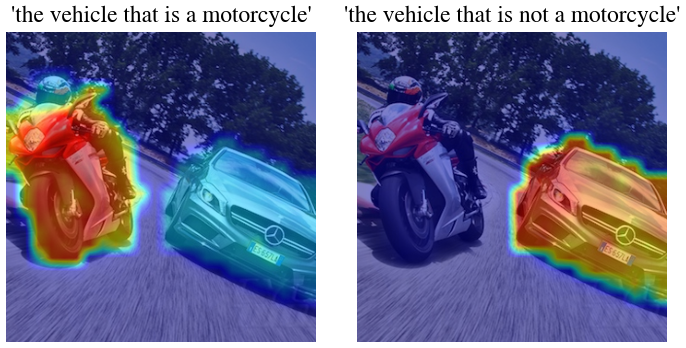
\includegraphics[width=0.63\linewidth]{figures/negation_heatmaps.png}
\hfill
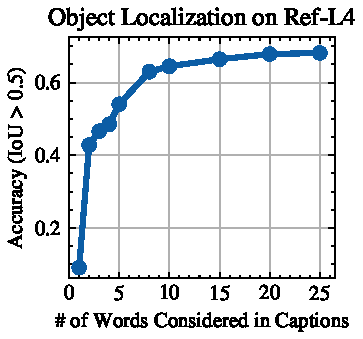
\includegraphics[width=0.35\linewidth]{figures/ref_l4_effective_token_length.pdf}

% \caption{Varying text complexity with negation (left) and length (right).}
\caption{Prompt Complexity: Negation changes the localized object (left). More detailed descriptions improve localization performance (right).}
\label{fig:negation_token_length}
\end{figure}

\paragraph{Presentation clarity.}
We thank \R1 and \R2 for highlighting clarity issues. We improved Fig.~3. 
For \R2, the linear-probe and ADE20k results are in the supplement but we will restore the omitted ADE20k column in Tab.~3.
We will also specify the used configuration (DINOv2 ViT-B/14 with $\omega{=}1$) earlier in §4 and clarify that only Fig.~2/Fig.~7 vary the learned gates post-hoc.
% We will also state the default SteerViT configuration (DINOv2 ViT-B/14 with $\omega{=}1$) upfront instead of in §4.7. This will also clarify that only Fig.~2/Fig.~7 vary the learned gates post-hoc, resulting in additional variants of the same model.



% ##########################################################################################

\clearpage


\begin{table}[t]
\centering
\footnotesize
\setlength{\tabcolsep}{3pt}

\caption{TODO.}
\label{tab:feature_preservation_old}

% \renewcommand{\arraystretch}{0.92}
\resizebox{\linewidth}{!}{
\begin{tabular}{@{}l c c c c c c c@{}}
\toprule
\textbf{Model} &
\multicolumn{3}{c}{\textbf{Classification}} &
\multicolumn{2}{c}{\textbf{Segmentation}} &
\multicolumn{2}{c}{\textbf{Action Recognition}} \\
\cmidrule(lr){2-4}\cmidrule(lr){5-6}\cmidrule(l){7-8}
& Birds & Cars & Dogs & ADE20k & City. & UCF101 & HMDB51 \\
\midrule
DINOv2                  & 94.7 & 83.8 & 89.1 & 53.7 & 52.8 & 92.3 & 62.3 \\
SteerViT ($\omega=0$)   & 94.7 & 83.8 & 89.1 & 53.7 & 52.8 & 92.3 & 62.3 \\
\rowcolor{\methodcolor} SteerViT ($\omega=1$)   & 91.2 & 77.7 & 94.3 & 55.4 & 53.8 & 89.4 & 60.0 \\
\bottomrule
\end{tabular}
}
\end{table}


\begin{table}[t]
\centering
\footnotesize
\setlength{\tabcolsep}{3pt} % default is usually 6pt
% \renewcommand{\arraystretch}{0.92}

\caption{Comparison of compute and multi-modal data efficiency.}
\label{tab:efficiency_old} 

\resizebox{\linewidth}{!}{
\begin{tabular}{@{}l c c c r r r@{}}
\toprule
\multicolumn{2}{c}{\textbf{Method}} &
\multicolumn{2}{c}{\textbf{MM Training}} &
\multicolumn{3}{c}{\textbf{Inference}} \\
\cmidrule(lr){1-2}\cmidrule(lr){3-4}\cmidrule(l){5-7}
Name & Params & Tuned \Fire & Samples &
\shortstack[c]{Compute\\[-1pt]{\scriptsize GFLOPS/img}} &
\shortstack[c]{Latency\\[-1pt]{\scriptsize ms/img}} &
\shortstack[c]{Memory\\[-1pt]{\scriptsize peak GiB}} \\
\midrule
CLIP          & 150M & all & 400M  & 81.4   & 5.5  & 1.1  \\
DINOv2        & 86M  & n/a & n/a   & 98.6   & 6.6  & 1.0  \\
\rowcolor{\methodcolor} SteerViT      & 465M & GCA & 2.28M & 133.8  & 9.5  & 3.0  \\
GroundDINO    & 172M & all & 5.4M  & 515.0  & 59.7 & 16.3 \\
SAM3          & 840M & all & 146M  & 556.0  & 35.1 & 5.3  \\
InternVL3-1B  & 938M & all & n/r   & 931.8  & 8.3  & 3.9  \\
InternVL3-2B  & 2.1B & all & n/r   & 1591.0 & 12.2 & 6.3  \\
\bottomrule
\end{tabular}
}
\end{table}

{
    \small
    \bibliographystyle{splncs04}
    \bibliography{bib/main}
}
\clearpage

% ---------------------------------------------------------------
% TODO REBUTTAL: Enter your response below
\section{Introduction}

After receiving paper reviews, the authors may optionally submit a rebuttal to address the reviewers' comments, which will be limited to a {\bf one page} PDF file.
Please follow the steps and style guidelines outlined below for submitting your author response.

The author rebuttal is optional and, following similar guidelines to previous conferences, is meant to provide you with an opportunity to rebut factual errors or to supply additional information requested by the reviewers.
It is NOT intended to add new contributions (theorems, algorithms, experiments) that were absent in the original submission and NOT specifically requested by the reviewers.
You may optionally add a figure, graph, table, or proof to your rebuttal to better illustrate your answer to the reviewers' comments.

Consistent with established practices in computer vision, reviewers should refrain from requesting significant additional experiments for the rebuttal or penalize for lack of additional experiments.
Authors should refrain from including new experimental results in the rebuttal, especially when not specifically requested to do so by the reviewers.
Authors may include figures with illustrations or comparison tables of results reported in the submission/supplemental material or in other papers.

Just like the original submission, the rebuttal must maintain anonymity.
Note that the rebuttal must not include external links.
The rebuttal must comply with this template (the use of sections is not required, though recommended to structure the rebuttal for ease of reading).
The rebuttal must also include line numbers as in this example document.
This allows for easy referencing of your response by reviewers and area chairs.


%-------------------------------------------------------------------------
\subsection{Response length}
Author responses must be no longer than 1 page in length including any references and figures.
Overlength responses will simply not be reviewed.
This includes responses where the margins and formatting are deemed to have been significantly altered from those laid down by this style guide.
Note that this \LaTeX\ guide already sets figure captions and references in a smaller font.


%------------------------------------------------------------------------
\section{Formatting your Response}

{\bf Make sure to update the paper title and paper ID in the appropriate place in the \verb+tex+ file.}

All text must be in a two-column format.
The total allowable size of the text area is $6\frac78$ inches (17.46 cm) wide by $8\frac78$ inches (22.54 cm) high.
Columns are to be $3\frac14$ inches (8.25 cm) wide, with a $\frac{5}{16}$ inch (0.8 cm) space between them.
The top margin should begin 1 inch (2.54 cm) from the top edge of the page.
The bottom margin should be $1\frac{1}{8}$ inches (2.86 cm) from the bottom edge of the page for $8.5 \times 11$-inch paper;
for A4 paper, approximately $1\frac{5}{8}$ inches (4.13 cm) from the bottom edge of the page.

Please number any displayed equations.
It is important for readers to be able to refer to any particular equation.

Wherever Times is specified, Times Roman may also be used.
The main text should be in 10-point Times, single-spaced.
Section headings should be in 10 or 12 point Times.
All paragraphs should be indented 1 pica (approx.\ $\frac{1}{6}$ inch or 0.422 cm).
Figure and table captions should be 9-point Roman type as in \cref{fig:onecol}.


List and number all bibliographical references in 9-point Times, single-spaced,
at the end of your response.
When referenced in the text, enclose the citation number in square brackets, for example~\cite{Alpher05}.
Where appropriate, include the name(s) of editors of referenced books.

\begin{figure}[t]
  \centering
  \fbox{\rule{0pt}{0.5in} \rule{0.9\linewidth}{0pt}}
  %\includegraphics[width=0.8\linewidth]{egfigure.eps}
   \caption{Example of caption.  It is set in Roman so that mathematics
   (always set in Roman: $B \sin A = A \sin B$) may be included without an
   ugly clash.}
   \label{fig:onecol}
\end{figure}

To avoid ambiguities, it is best if the numbering for equations, figures, tables, and references in the author response does not overlap with that in the main paper (the reviewer or AC may wonder if you talk about \cref{fig:onecol} in the author response or in the actual paper).
See the \LaTeX\ source of the rebuttal template for a workaround.


%-------------------------------------------------------------------------
\subsection{Illustrations, graphs, and photographs}

Please ensure that any point you wish to make is resolvable in a printed copy of the response.
Resize fonts in figures to at least 6\:pt ($\sim$2\:mm character height), and choose line widths that render effectively in print.
Readers (and reviewers/ACs), even of an electronic copy, may choose to print your response in order to read it.
You cannot insist that they do otherwise, and therefore must not assume that they can zoom in to see tiny details on a graphic.


%-------------------------------------------------------------------------
% References



\end{document}
